\section{Introduction: a framework for AI-assisted TPC research}
The twin-prime problem asks for infinitely many prime pairs at the fixed displacement $2$. For an AI assistant working across a long research archive, even identifying the next legitimate task requires more than retrieving a plausible formula. The assistant must recover the exact object, distinguish a proved statement from a proposed transfer, and retain the hypotheses that connect local work to the arithmetic endpoint. A change of variables may preserve every coefficient without producing cancellation. A small normalized matrix may carry large coefficient costs. A full-measure recurrence theorem may omit the one initial point that encodes the integers. Losing these distinctions can make an apparently coherent continuation address a different problem.

We therefore present a source-traceable, file-based research framework: an existing mathematical archive and linked knowledge base, a specification for AI-facing source and task records, and a prospective evaluation agenda. Its purpose is to support human-supervised research on a difficult open problem while making object changes, unpaid losses, and unresolved obligations explicit. The mathematical synthesis is the worked case through which these requirements become concrete. The framework is not a general autonomous research engine, and its effects on model reliability or research efficiency have not been measured.

We use the seven-island map in Figure~\ref{fig:map} to separate arithmetic foundations, analytic cancellation, fixed atoms, actual occurrences, moving-target dynamics, the twin-prime endpoint, and auxiliary geometric lifts. The islands are not successive steps of a proved implication. We reconstruct selected results by their dependencies, rather than by the order of the archived investigations. This is neither a claim of first discovery nor an exhaustive account of every route to twin primes.

\subsection{Three contributions and their evidence levels}
First, we provide a source-traceable mathematical synthesis with explicit proofs, transfer requirements, and unresolved endpoints. Second, we connect the existing source archive and research wiki to a bounded AI task protocol: what to read, which object and hypotheses to preserve, what evidence to return, and who may accept a proposed continuation. The companion framework source map distinguishes already present metadata and safeguards from fields proposed for standardization. Third, we formulate a research agenda and a controlled evaluation design. The archive and wiki are concrete artifacts; a fully automated workflow and demonstrated AI benefits are not results of this paper.

The formal mathematics ecosystem addresses a related but different layer. The Lean mathematical library provides formalized mathematics, while LeanDojo supplies infrastructure and a benchmark for learning-based theorem proving in Lean~\cite{mathlib2019,yang2023leandojo}. Our emphasis is upstream informal research organization: selecting source-grounded tasks and preventing unsupported transfers between mathematical settings. This framework neither replaces proof checking nor formally verifies the TPC archive. Selective formalization is a proposed extension, and systematic positioning against other AI-research systems remains future work.

\subsection{Two gaps, with different endpoint connections}
The analytic core concerns a specific mixed scalar $\Cx=\ip w{A\beta}$, of natural scale $xQ^2$. The vectors, unit masks, physical interval, Fourier convention, and deleted diagonal are part of its definition. A full-scalar saving with exponent strictly greater than $1/400$ would be useful in the imported analytic interface, but that interface also requires a separate full-shell estimate called Gate A. Both gates lie inside map Bridge A. Their conditional output in this paper is a bound for another auxiliary scalar, $S_x^{\rm phys}$; the complete upstream implication to prime-pair counting is not reproved here.

The dynamical connection is pointwise and explicit: the moving sieve events at seed $0$ identify the pairs $n,n+2$ that are both prime. Adequate mass and covariance control do prove infinite recurrence for almost every seed. They do not establish that the prescribed seed belongs to that good set. Map Bridge B names this return to the distinguished arithmetic point. An auxiliary geometric representation must preserve the same event and seed correspondence; changing the ambient space alone cannot close the gap.

\subsection{Results and their roles}
The main results serve distinct roles. Proposition~\ref{prop:decomp} identifies the exact positive-form structure behind the actual operator. Theorem~\ref{thm:normbarrier}, Corollary~\ref{cor:normalized}, and Theorem~\ref{thm:rank} delimit coefficient-blind norm bounds and low-rank repairs. Proposition~\ref{prop:emitter} identifies the complete Kloosterman arrays, whereas Condition~\ref{cond:compression} states an unproved, loss-controlled attachment to a two-sided short-array estimate. Theorem~\ref{thm:boundary} supplies a genuine bound for one component of the original scalar. Finally, Theorem~\ref{thm:haar} proves metric recurrence for the actual moving targets, and Proposition~\ref{prop:seed} isolates a sufficient, still-unverified way to reach seed $0$.

The distinction between these roles matters. A method obstruction is not a lower bound for the actual scalar. A boundary estimate is not an interior estimate. A sufficient criterion is not a verified hypothesis. In particular, the fixed-atom and occurrence interfaces in Section~\ref{sec:structure} explain what an arithmetic attachment must preserve; they do not construct all the upstream attachments needed by the analytic program.

\subsection{Mathematical inputs and scope}
Our prime-counting input is the classical prime number theorem and its partial-summation consequences~\cite{selberg1949}. The hybrid coefficient's second-moment estimate uses the unconditional Mertens product baseline stated at the beginning of~\cite{lamzouri2015}; none of that paper's conditional bias-distribution results is used. Frequency separation, positive-semidefinite compression, finite Fourier orthogonality, and spectral min--max arguments provide the structural tools.

The critical-interval bilinear estimate of Blomer--Pascadi~\cite{blomer2026} supplies an external benchmark. Its square-root-length specialization offers a local Kloosterman saving under specified support and coprimality conditions. Our question is whether the actual signed expression can be attached to those inputs with all losses paid. The external theorem does not itself provide that attachment.

The source-linked research wiki~\cite{archiveframework} organizes distinctions between definitions, estimates, obstructions, and conditional transfers. It is a secondary reading aid, not independent evidence for a theorem. The original proofs remain the mathematical sources; Appendix~\ref{sec:provenance} and the companion concordance explain how to locate them. A systematic external literature comparison and novelty assessment remain necessary before submission.

\subsection{Reading guide}
Section~\ref{sec:framework} specifies the AI-facing framework. Sections~\ref{sec:arithmetic}--\ref{sec:structure} fix the arithmetic endpoint and structural interfaces. Sections~\ref{sec:operator}--\ref{sec:boundary} develop the analytic case; Section~\ref{sec:dynamics} treats metric recurrence and the distinguished seed. Section~\ref{sec:bridges} collects the remaining obligations, and Section~\ref{sec:agenda} gives the research agenda. The branches can be read separately; the companion source records provide exact locators.

\clearpage
\begin{figure}[p]
\centering
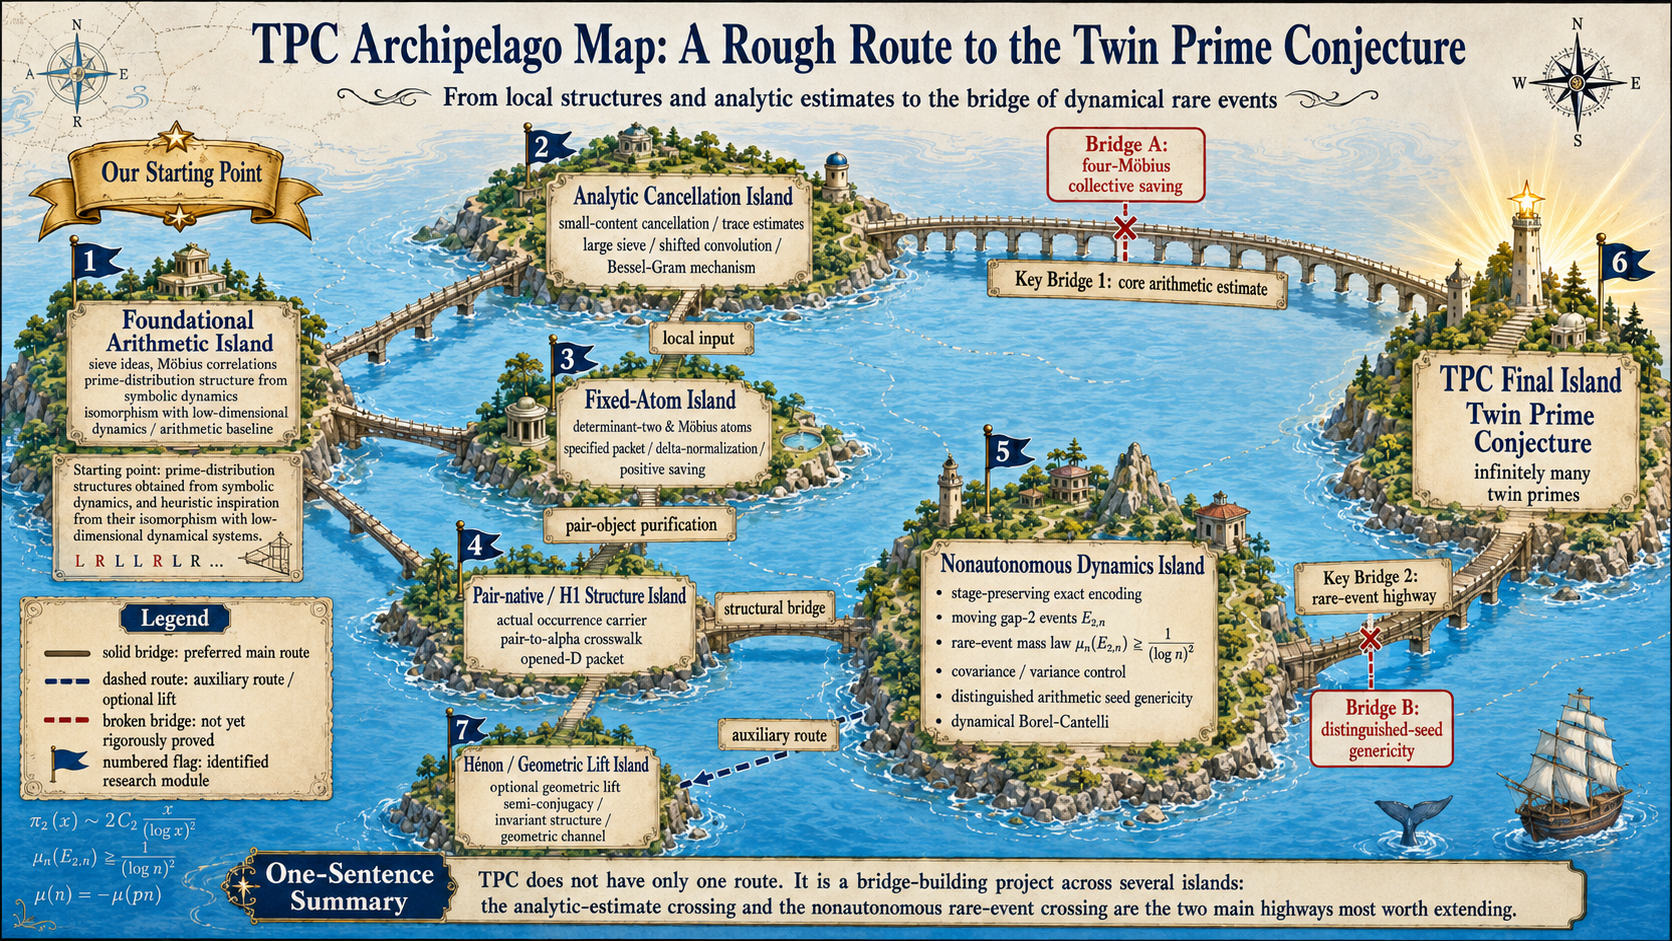
\includegraphics[width=\textwidth]{figures/tpc_route_en.png}
\caption{The user's seven-island map, reproduced unchanged. Islands name objects and tasks, not completed steps. Connections are proposed routes, not certified implications; broken bridges mark unproved transfers, not universal impossibility. Schematic formulae do not establish isomorphisms, savings, or prime-pair asymptotics: the hypotheses in the text govern those claims. Map Bridge A contains both analytic Gate A and Gate B; map Bridge B concerns the distinguished arithmetic seed. Rare-event mass alone does not establish recurrence at that seed. The full-resolution companion preserves the small labels for enlargement.}
\label{fig:map}
\end{figure}
\clearpage
